\documentclass[12pt,a4paper]{article}

% ── Packages ──────────────────────────────────────────────
\usepackage[utf8]{inputenc}
\usepackage[T1]{fontenc}
\usepackage{lmodern}
\usepackage[margin=2.5cm]{geometry}
\usepackage{graphicx}
\usepackage{xcolor}
\usepackage{listings}
\usepackage{hyperref}
\usepackage{booktabs}
\usepackage{float}
\usepackage{enumitem}
\usepackage{caption}
\usepackage{parskip}
\usepackage{fancyhdr}
\usepackage{titlesec}

% ── Colors ────────────────────────────────────────────────
\definecolor{codeblue}{RGB}{26,54,93}
\definecolor{codegray}{RGB}{100,100,100}
\definecolor{codegreen}{RGB}{22,101,52}
\definecolor{codepurple}{RGB}{128,0,128}
\definecolor{backcolor}{RGB}{248,250,252}
\definecolor{stringcolor}{RGB}{163,21,21}

% ── Code Listing Style ───────────────────────────────────
\lstdefinestyle{codestyle}{
    backgroundcolor=\color{backcolor},
    commentstyle=\color{codegreen},
    keywordstyle=\color{codeblue}\bfseries,
    stringstyle=\color{stringcolor},
    basicstyle=\ttfamily\scriptsize,
    breakatwhitespace=false,
    breaklines=true,
    captionpos=b,
    keepspaces=true,
    showspaces=false,
    showstringspaces=false,
    showtabs=false,
    tabsize=2,
    frame=single,
    rulecolor=\color{codegray!30},
    xleftmargin=1em,
    framexleftmargin=0.5em,
    numbers=left,
    numberstyle=\tiny\color{codegray},
    numbersep=8pt,
}
\lstset{style=codestyle}

% TypeScript language definition for listings
\lstdefinelanguage{TypeScript}{
  keywords={const, let, var, function, return, if, else, for, while, do, switch, case, break, continue, new, try, catch, throw, typeof, instanceof, in, of, class, extends, implements, interface, type, enum, import, export, from, default, as, async, await, yield, true, false, null, undefined, void, never, any, string, number, boolean, object},
  sensitive=true,
  comment=[l]{//},
  morecomment=[s]{/*}{*/},
  morestring=[b]",
  morestring=[b]',
  morestring=[b]`,
}

% ── Section Styling ───────────────────────────────────────
\titleformat{\section}{\Large\bfseries\color{codeblue}}{\thesection}{1em}{}
\titleformat{\subsection}{\large\bfseries\color{codeblue!80}}{\thesubsection}{1em}{}
\titleformat{\subsubsection}{\normalsize\bfseries\color{codeblue!60}}{\thesubsubsection}{1em}{}

% ── Header / Footer ──────────────────────────────────────
\pagestyle{fancy}
\fancyhf{}
\fancyhead[L]{\small\textit{Sakny — University Housing Platform}}
\fancyhead[R]{\small\textit{Frontend Implementation}}
\fancyfoot[C]{\thepage}
\renewcommand{\headrulewidth}{0.4pt}

% ── Document ─────────────────────────────────────────────
\begin{document}

% ══════════════════════════════════════════════════════════
% TITLE
% ══════════════════════════════════════════════════════════
\begin{center}
    {\LARGE\bfseries\color{codeblue} Frontend Implementation}\\[0.5em]
    {\large Sakny — University Housing Platform}\\[1em]
    \rule{0.6\textwidth}{0.5pt}
\end{center}

\tableofcontents
\newpage

% ══════════════════════════════════════════════════════════
% SECTION 1: INTRODUCTION & TECHNOLOGY STACK
% ══════════════════════════════════════════════════════════
\section{Introduction \& Technology Stack}

The Sakny frontend is a modern web application that serves as the primary interface for the university housing platform. It provides two main portals: a \textbf{Student Portal} where students can apply for housing, upload documents, track their application status, communicate with administrators, and manage their accommodation; and an \textbf{Admin Portal} where housing administrators can review applications, manage room allocations, handle maintenance tickets, and monitor system-wide analytics.

The frontend was designed with a focus on component reusability, type safety, bilingual support (English/Arabic with RTL), and a clean, maintainable codebase.

\subsection{Technology Stack}

\begin{table}[H]
\centering
\begin{tabular}{@{}llp{7cm}@{}}
\toprule
\textbf{Technology} & \textbf{Version} & \textbf{Role \& Justification} \\
\midrule
Next.js & 16.2.4 & React framework providing file-based routing via the App Router, nested layouts, server components, and built-in SEO metadata API. \\
React & 19.2.4 & Core UI library enabling a component-based architecture with hooks for state management and side effects. \\
TypeScript & 5.x & Adds static type checking across the entire codebase, catching errors at compile time and improving developer experience with IntelliSense. \\
Tailwind CSS & 4.x & Utility-first CSS framework allowing rapid UI development with a custom design token system for consistent styling. \\
Material Symbols & — & Google's icon library loaded via Google Fonts, providing 2,500+ icons used throughout the interface. \\
PostCSS & — & CSS processing pipeline required by Tailwind CSS for compilation. \\
\bottomrule
\end{tabular}
\caption{Frontend technology stack.}
\end{table}

% ══════════════════════════════════════════════════════════
% SECTION 2: PROJECT STRUCTURE
% ══════════════════════════════════════════════════════════
\section{Project Structure \& File Organization}

The frontend follows a clear separation of concerns, organizing code by responsibility. The \texttt{src/} directory is divided into five top-level folders, each with a distinct purpose:

\begin{lstlisting}[language={},title={Project folder structure}]
src/
|-- app/                    # Pages & Layouts (Next.js App Router)
|   |-- layout.tsx          # Root layout (fonts, providers, metadata)
|   |-- page.tsx            # Landing page
|   |-- auth/               # Authentication page
|   |-- dashboard/          # Student portal (14 sub-routes)
|   |-- admin/              # Admin portal (13 sub-modules)
|-- components/             # Reusable UI components
|   |-- ui/                 # Primitives (Button, Card, FormField, ...)
|   |-- auth/               # Auth-specific (LoginForm, RegisterForm, ...)
|   |-- dashboard/          # Dashboard (Sidebar, Navbar, Stepper, ...)
|   |-- admin/              # Admin (AdminSidebar)
|-- services/               # API communication layer
|   |-- api.ts              # Centralized API client
|-- hooks/                  # Custom React hooks
|   |-- useScrollReveal.ts  # Intersection Observer for animations
|-- i18n/                   # Internationalization (Arabic/English)
    |-- LanguageContext.tsx  # Language provider
    |-- useTranslation.ts   # Translation hook
    |-- locales/            # Translation JSON files (en.json, ar.json)
\end{lstlisting}

\textbf{Key design decisions:}
\begin{itemize}[leftmargin=2em]
    \item \texttt{app/} contains only pages and layouts — no business logic or UI components.
    \item \texttt{components/ui/} acts as the design system primitives layer. Every form input, button, and card across the app is built from these 6 base components.
    \item Components are domain-grouped (\texttt{auth/}, \texttt{dashboard/}, \texttt{admin/}) rather than flat, making it clear which feature area each component belongs to.
    \item \texttt{services/api.ts} is the single point of contact with the backend — no component calls \texttt{fetch()} directly.
\end{itemize}

% ══════════════════════════════════════════════════════════
% SECTION 3: DESIGN SYSTEM & STYLING
% ══════════════════════════════════════════════════════════
\section{Design System \& Styling Approach}

The visual language of the application is built on Tailwind CSS with a custom \textbf{design token system} defined in \texttt{globals.css}. This ensures consistent colors, typography, and spacing across all pages.

\subsection{Design Tokens}

\begin{lstlisting}[language=TypeScript,title={globals.css — Custom design tokens (trimmed)}]
@import "tailwindcss";

@theme {
  /* Primary palette */
  --color-primary: #1A365D;
  --color-primary-container: #152c4d;
  --color-accent-yellow: #FBBF24;
  --color-background: #F8FAFC;
  --color-surface: #ffffff;

  /* Status colors */
  --color-status-available: #166534;
  --color-status-limited: #a16207;
  --color-status-full: #991b1b;

  /* Typography */
  --font-headline: "Manrope", sans-serif;
  --font-body: "Public Sans", sans-serif;

  /* Shadows */
  --shadow-soft: 0 4px 20px -2px rgba(0, 0, 0, 0.05);
  --shadow-soft-lg: 0 10px 30px -5px rgba(0, 0, 0, 0.08);
}
\end{lstlisting}

\textbf{Semantic naming:} Instead of using raw hex values throughout the codebase, every color is referenced by its semantic role (e.g., \texttt{text-primary}, \texttt{bg-surface}, \texttt{text-status-available}). This makes the design easy to update globally by changing a single token value.

The token system follows the \textbf{Material Design 3} surface hierarchy (\texttt{surface-container-low}, \texttt{surface-container-high}, etc.) for layered elevation effects in the dashboard.

\subsection{Typography}

Fonts are loaded using Next.js's built-in \texttt{next/font} module, which automatically optimizes font loading and eliminates layout shift:

\begin{lstlisting}[language=TypeScript,title={layout.tsx — Font loading with CSS variables}]
const manrope = Manrope({
  subsets: ["latin"],
  variable: "--font-headline",
  display: "swap",
});

const publicSans = Public_Sans({
  subsets: ["latin"],
  variable: "--font-body",
  display: "swap",
});
\end{lstlisting}

\textbf{Manrope} is used for headlines and navigation, while \textbf{Public Sans} is used for body text, labels, and form inputs.

\subsection{Custom Utilities}

Two custom Tailwind utilities are defined for specialized visual effects:

\begin{lstlisting}[language=TypeScript,title={Glassmorphism navbar utility}]
@utility glass-nav {
  background-color: rgba(255, 255, 255, 0.9);
  backdrop-filter: blur(16px);
  -webkit-backdrop-filter: blur(16px);
}
\end{lstlisting}

The \texttt{glass-nav} utility creates a frosted-glass effect on the navigation bar, allowing background content to subtly show through while maintaining readability.

% ══════════════════════════════════════════════════════════
% SECTION 4: ROUTING & PAGE MANAGEMENT
% ══════════════════════════════════════════════════════════
\section{Routing \& Page Management}

The application uses Next.js \textbf{App Router}, which provides file-system-based routing. Each folder inside \texttt{app/} automatically becomes a URL route, and each \texttt{page.tsx} file becomes the page rendered at that route.

\subsection{Route Map}

The application contains 30+ routes organized into three main sections:

\begin{figure}[H]
    \centering
    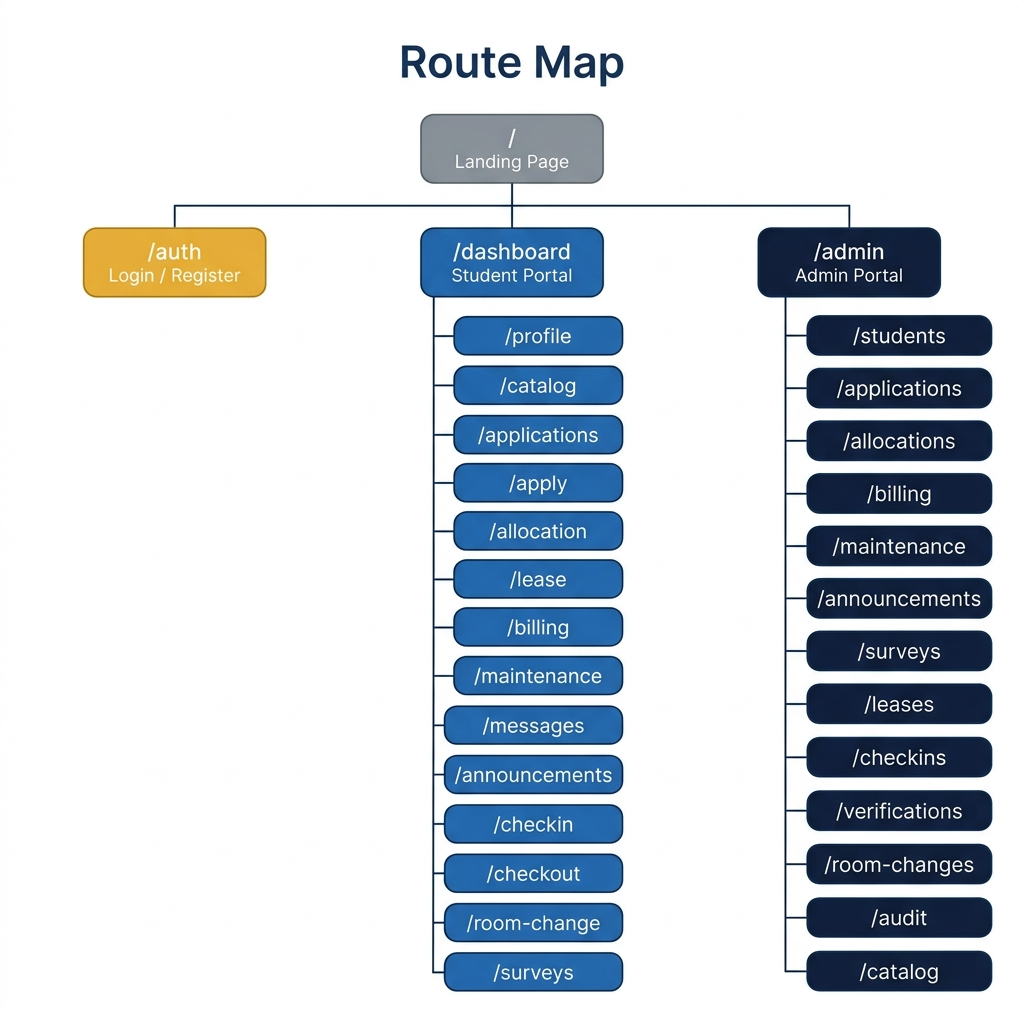
\includegraphics[width=\textwidth]{images/route_map_diagram.png}
    \caption{Complete route map of the Sakny frontend application.}
\end{figure}

\begin{table}[H]
\centering
\small
\begin{tabular}{@{}lll@{}}
\toprule
\textbf{Route} & \textbf{Section} & \textbf{Purpose} \\
\midrule
\texttt{/} & Landing & Public marketing page \\
\texttt{/auth} & Authentication & Login / Register forms \\
\texttt{/dashboard} & Student & Student home with document status \\
\texttt{/dashboard/catalog} & Student & Browse available housing \\
\texttt{/dashboard/applications} & Student & Track applications \\
\texttt{/dashboard/messages} & Student & Send/receive messages \\
\texttt{/dashboard/billing} & Student & View payments \\
\texttt{/admin} & Admin & Analytics dashboard \\
\texttt{/admin/students} & Admin & Student management \\
\texttt{/admin/applications} & Admin & Review applications \\
\texttt{/admin/maintenance} & Admin & Ticket management \\
\bottomrule
\end{tabular}
\caption{Key routes (partial list — 30+ routes total).}
\end{table}

\subsection{Nested Layouts}

Next.js App Router supports \textbf{nested layouts}, where a parent layout wraps all child pages. This eliminates the need to repeat shared UI elements (navbar, sidebar) on every page.

\begin{figure}[H]
    \centering
    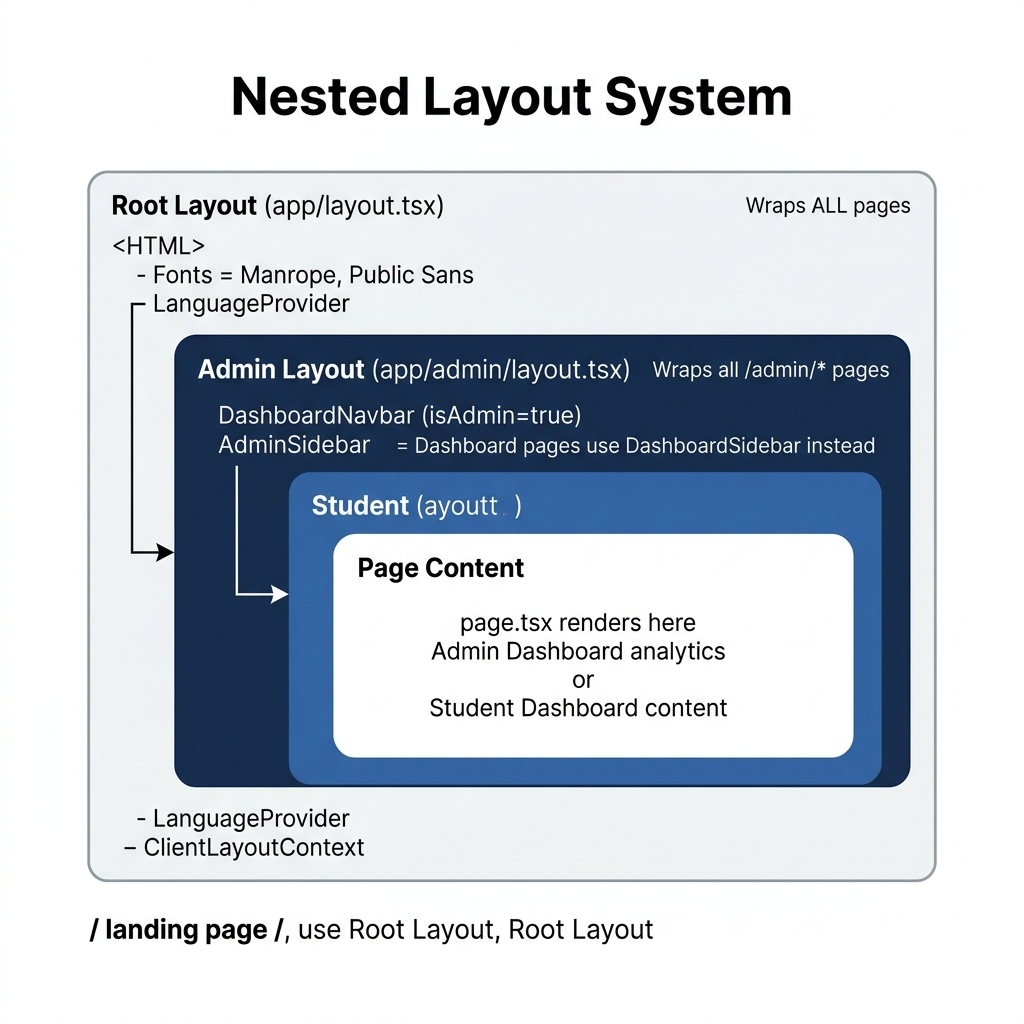
\includegraphics[width=0.85\textwidth]{images/nested_layouts.png}
    \caption{Nested layout inheritance — Root Layout wraps all pages, Admin Layout adds sidebar and navbar.}
\end{figure}

\textbf{Root Layout} (\texttt{app/layout.tsx}) — wraps every page in the application:

\begin{lstlisting}[language=TypeScript,title={Root layout — Provider wrapping pattern}]
export default function RootLayout({ children }) {
  return (
    <html lang="en" className={`${manrope.variable} ${publicSans.variable}`}>
      <body>
        <LanguageProvider>
          <ClientLayoutContext>
            {children}
          </ClientLayoutContext>
        </LanguageProvider>
      </body>
    </html>
  );
}
\end{lstlisting}

\textbf{Admin Layout} (\texttt{app/admin/layout.tsx}) — adds the admin sidebar and navbar for all \texttt{/admin/*} pages:

\begin{lstlisting}[language=TypeScript,title={Admin nested layout}]
export default function AdminLayout({ children }) {
  return (
    <div className="min-h-screen flex flex-col">
      <DashboardNavbar isAdmin />
      <AdminSidebar />
      <main className="lg:ml-64 pt-24 pb-12 px-8 flex-grow">
        {children}
      </main>
    </div>
  );
}
\end{lstlisting}

\subsection{Server Components vs Client Components}

Next.js App Router uses \textbf{Server Components} by default. Components that need browser APIs (event handlers, \texttt{useState}, \texttt{useEffect}, \texttt{localStorage}) must be marked with the \texttt{"use client"} directive at the top of the file. In our project, all interactive components use \texttt{"use client"}, while page wrappers and layouts that only define metadata remain as server components.

% ══════════════════════════════════════════════════════════
% SECTION 5: REUSABLE COMPONENT DESIGN
% ══════════════════════════════════════════════════════════
\section{Reusable Component Design}

The component architecture follows a three-layer composition model: \textbf{UI Primitives} are composed into \textbf{Feature Components}, which are assembled into \textbf{Pages}.

\begin{figure}[H]
    \centering
    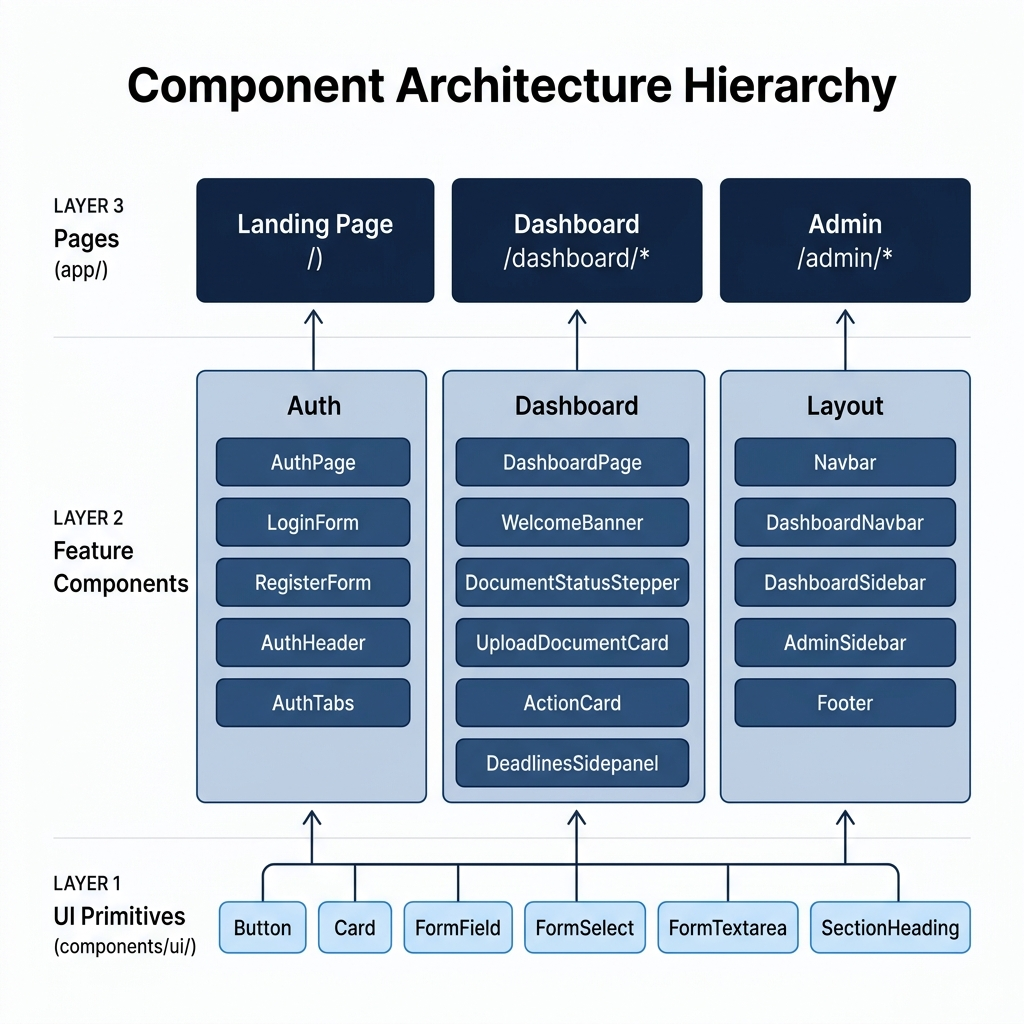
\includegraphics[width=\textwidth]{images/component_hierarchy.png}
    \caption{Component hierarchy — primitives compose into feature components, which compose into pages.}
\end{figure}

\subsection{UI Primitives (\texttt{components/ui/})}

Six base components form the design system:

\begin{table}[H]
\centering
\begin{tabular}{@{}llp{6.5cm}@{}}
\toprule
\textbf{Component} & \textbf{Key Props} & \textbf{Purpose} \\
\midrule
\texttt{Button} & \texttt{variant}, \texttt{icon}, \texttt{iconPosition} & Multi-variant button (primary, secondary, outline, navy) \\
\texttt{Card} & \texttt{icon}, \texttt{title}, \texttt{description} & Feature display card with icon and link \\
\texttt{FormField} & \texttt{label}, \texttt{icon}, \texttt{error} & Text input with validation, password toggle, RTL support \\
\texttt{FormSelect} & \texttt{label}, \texttt{options}, \texttt{error} & Dropdown select with validation \\
\texttt{FormTextarea} & \texttt{label}, \texttt{error} & Multi-line text input \\
\texttt{SectionHeading} & title text & Styled section title \\
\bottomrule
\end{tabular}
\caption{UI primitive components.}
\end{table}

\subsubsection{Button Component — Variant Map Pattern}

The \texttt{Button} component demonstrates a key design pattern: the \textbf{variant map}, where each visual style is defined as a string of Tailwind classes mapped to a variant name:

\begin{lstlisting}[language=TypeScript,title={Button.tsx — Variant map pattern (key parts)}]
type ButtonProps = React.ButtonHTMLAttributes<HTMLButtonElement> & {
  variant?: "primary" | "secondary" | "outline" | "navy";
  icon?: string;
  iconPosition?: "left" | "right";
};

export const Button: React.FC<ButtonProps> = ({
  variant = "primary", icon, iconPosition = "right",
  children, className = "", ...props
}) => {
  const variants = {
    primary: "bg-accent-yellow text-primary rounded-xl font-bold ...",
    secondary: "bg-white/10 backdrop-blur-md text-white ...",
    outline: "bg-surface border border-slate-200 ...",
    navy: "bg-primary text-white rounded-lg ...",
  };

  return (
    <button className={`${baseStyles} ${variants[variant]} ${className}`}
            {...props}>
      {icon && iconPosition === "left" && (
        <span className="material-symbols-outlined">{icon}</span>
      )}
      {children}
      {icon && iconPosition === "right" && (
        <span className="material-symbols-outlined">{icon}</span>
      )}
    </button>
  );
};
\end{lstlisting}

The component extends native HTML button attributes via \texttt{React.ButtonHTMLAttributes}, allowing any standard HTML attribute (\texttt{disabled}, \texttt{type}, \texttt{onClick}) to be passed through without explicit prop definitions.

\subsubsection{FormField Component — Validation \& RTL Support}

The \texttt{FormField} component handles text inputs with built-in support for error states, password visibility toggling, and RTL layout:

\begin{lstlisting}[language=TypeScript,title={FormField.tsx — Key features}]
export const FormField: React.FC<FormFieldProps> = ({
  label, icon, error, type = "text", ...props
}) => {
  const [showPassword, setShowPassword] = useState(false);
  const isPassword = type === "password";
  const currentType = isPassword && showPassword ? "text" : type;

  return (
    <div className="flex flex-col gap-1.5 w-full">
      <label className="font-label font-semibold text-sm text-primary">
        {label}
      </label>
      <div className="relative flex items-center rtl:flex-row-reverse">
        {icon && (
          <span className="absolute left-4 rtl:left-auto rtl:right-4">
            {icon}
          </span>
        )}
        <input
          type={currentType}
          className={`w-full border ${
            error ? "border-red-500 ring-2 ring-red-500/20"
                  : "border-slate-200"
          } rounded-lg ...`}
          {...props}
        />
      </div>
      {error && <span className="text-red-500 text-xs">{error}</span>}
    </div>
  );
};
\end{lstlisting}

Note the \texttt{rtl:} prefix classes — these are Tailwind's RTL modifiers that activate only when the page direction is right-to-left (Arabic), automatically flipping icon positions and padding.

\subsection{Feature Components — Composition}

Feature components compose the primitives into complete UI sections. For example, the \texttt{LoginForm} combines \texttt{FormField} and \texttt{Button}:

\begin{lstlisting}[language=TypeScript,title={LoginForm.tsx — Composing primitives (key structure)}]
export const LoginForm: React.FC<LoginFormProps> = ({ onSwitchToRegister }) => {
  const { t, locale } = useTranslation();

  return (
    <form onSubmit={handleSubmit} className="flex flex-col gap-6">
      {apiError && (
        <div className="bg-red-50 text-red-600 p-3 rounded-lg">
          {apiError}
        </div>
      )}
      <FormField id="email" label={t("auth.fields.email")}
                 icon="mail" error={errors.email} ... />
      <FormField id="password" type="password"
                 label={t("auth.fields.password")} icon="lock" ... />
      <Button type="submit" variant="primary" icon="login"
              iconPosition={locale === "ar" ? "left" : "right"}>
        {t("auth.loginButton")}
      </Button>
    </form>
  );
};
\end{lstlisting}

\subsection{Layout Components}

Shared layout components provide consistent navigation across the application:

\begin{itemize}[leftmargin=2em]
    \item \textbf{DashboardNavbar} — Reused for both student and admin portals via an \texttt{isAdmin} prop. Shows notification badges with real-time polling, user avatar with dropdown, and active route display.
    \item \textbf{DashboardSidebar} — Data-driven navigation list with active-route highlighting using \texttt{usePathname()} from Next.js. Renders all 10 student navigation items from an array.
    \item \textbf{AdminSidebar} — Separate sidebar for the 13 admin modules.
\end{itemize}

The sidebar navigation is \textbf{data-driven}: items are defined as an array and rendered via \texttt{.map()}, making it easy to add or remove navigation items:

\begin{lstlisting}[language=TypeScript,title={DashboardSidebar.tsx — Data-driven navigation}]
const navItems = [
  { href: "/dashboard", icon: "dashboard", label: t("dashboard.sidebarHome") },
  { href: "/dashboard/profile", icon: "person", label: t("dashboard.sidebarProfile") },
  { href: "/dashboard/catalog", icon: "apartment", label: t("dashboard.sidebarCatalog") },
  // ... 7 more items
];

{navItems.map((item) => {
  const isActive = pathname === item.href ||
                   pathname?.startsWith(item.href + "/");
  return (
    <Link href={item.href}
          className={isActive ? "text-primary bg-primary-fixed/30"
                              : "text-on-surface-variant"}>
      <span className="material-symbols-outlined">{item.icon}</span>
      <span>{item.label}</span>
    </Link>
  );
})}
\end{lstlisting}

% ══════════════════════════════════════════════════════════
% SECTION 6: API INTEGRATION
% ══════════════════════════════════════════════════════════
\section{API Integration \& Backend Communication}

All communication with the backend REST API is routed through a single, centralized API client located in \texttt{services/api.ts}. No component calls \texttt{fetch()} directly — this ensures consistent error handling, authentication headers, and response parsing across the entire application.

\begin{figure}[H]
    \centering
    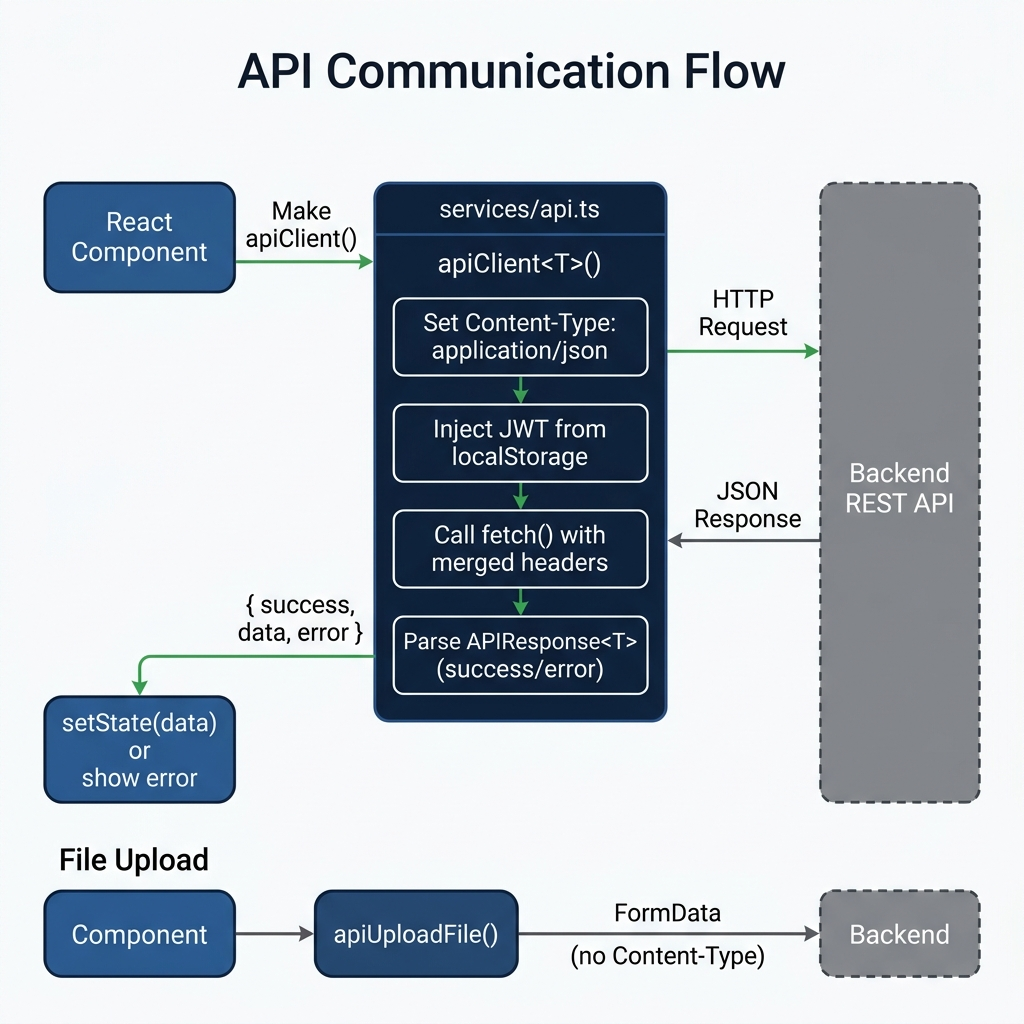
\includegraphics[width=\textwidth]{images/api_flow_diagram.png}
    \caption{API request flow — all requests go through the centralized apiClient.}
\end{figure}

\subsection{The \texttt{apiClient<T>()} Function}

\begin{lstlisting}[language=TypeScript,title={api.ts — Centralized API client (key parts)}]
export interface APIResponse<T = any> {
  success: boolean;
  data: T | null;
  error: string | null;
}

export const API_BASE_URL =
  process.env.NEXT_PUBLIC_API_URL || "http://localhost:8000/api/v1";

export async function apiClient<T>(
  endpoint: string,
  options: RequestInit = {}
): Promise<APIResponse<T>> {
  try {
    const defaultHeaders: HeadersInit = {
      "Content-Type": "application/json",
    };

    // Inject JWT token from localStorage
    if (typeof window !== "undefined") {
      const token = localStorage.getItem("access_token");
      if (token) {
        defaultHeaders.Authorization = `Bearer ${token}`;
      }
    }

    const response = await fetch(`${API_BASE_URL}${endpoint}`, {
      ...options,
      headers: { ...defaultHeaders, ...options.headers },
    });

    const data = await response.json();
    if (!response.ok) {
      return { success: false, data: null, error: data.error || "Request failed" };
    }
    return { success: true, data: data.data, error: null };
  } catch (error: any) {
    return { success: false, data: null, error: error.message || "Network error" };
  }
}
\end{lstlisting}

\textbf{Key design decisions:}
\begin{itemize}[leftmargin=2em]
    \item \textbf{Generic typing} (\texttt{<T>}) — allows each call site to specify the expected response type, providing full TypeScript autocomplete on the response data.
    \item \textbf{Automatic JWT injection} — every request automatically includes the Bearer token from \texttt{localStorage}, so components never need to manage authentication headers.
    \item \textbf{Unified response shape} — every API call returns \texttt{\{success, data, error\}}, making error handling consistent across all components.
    \item \textbf{Environment-based URL} — the base URL reads from \texttt{NEXT\_PUBLIC\_API\_URL}, allowing different URLs for development, staging, and production without code changes.
\end{itemize}

\subsection{Usage Example}

\begin{lstlisting}[language=TypeScript,title={Calling the API from a component}]
const response = await apiClient<any>("/auth/login", {
  method: "POST",
  body: JSON.stringify({ email, password }),
});

if (response.success && response.data) {
  localStorage.setItem("access_token", response.data.access_token);
  router.push("/dashboard");
} else {
  setApiError(response.error || "Login failed");
}
\end{lstlisting}

\subsection{File Upload Handler}

A separate \texttt{apiUploadFile<T>()} function handles \texttt{FormData} uploads. The key difference is that it does \textbf{not} set the \texttt{Content-Type} header — the browser automatically sets it with the correct multipart boundary when sending \texttt{FormData}.

% ══════════════════════════════════════════════════════════
% SECTION 7: AUTHENTICATION & AUTHORIZATION
% ══════════════════════════════════════════════════════════
\section{Authentication \& Authorization Flow}

The frontend implements a complete authentication lifecycle using JWT (JSON Web Tokens) stored in the browser's \texttt{localStorage}.

\begin{figure}[H]
    \centering
    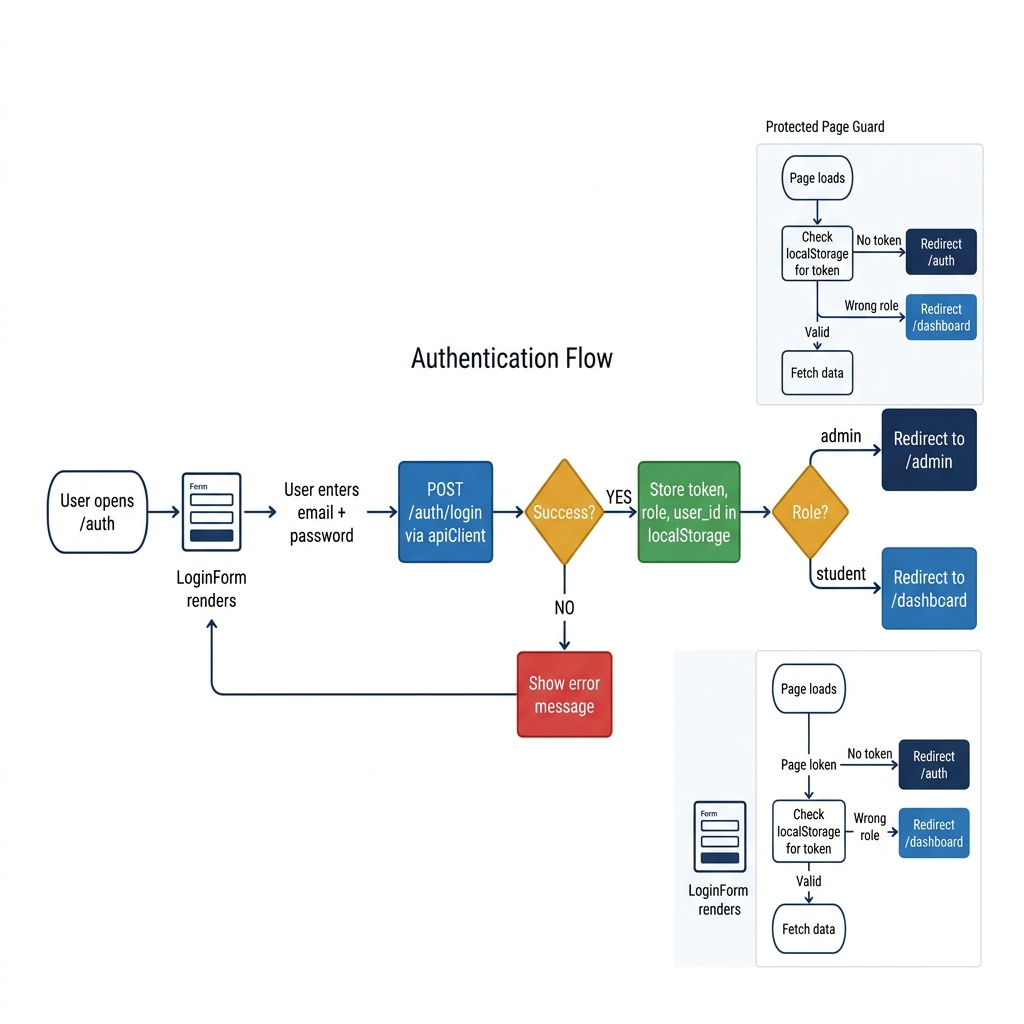
\includegraphics[width=\textwidth]{images/auth_flow_diagram.png}
    \caption{Authentication flow — from login to role-based routing to protected page guards.}
\end{figure}

\subsection{Login Flow}

When a user submits the login form:

\begin{enumerate}[leftmargin=2em]
    \item The \texttt{LoginForm} component sends a \texttt{POST /auth/login} request via \texttt{apiClient}.
    \item On success, the response contains an \texttt{access\_token}, \texttt{user\_role}, and \texttt{user\_id}.
    \item These values are stored in \texttt{localStorage} for persistence across page reloads.
    \item The user is redirected based on their role: \texttt{admin} $\rightarrow$ \texttt{/admin}, \texttt{student} $\rightarrow$ \texttt{/dashboard}.
\end{enumerate}

\subsection{Protected Page Guards}

Every protected page checks for authentication and authorization in a \texttt{useEffect} hook that runs on mount:

\begin{lstlisting}[language=TypeScript,title={Route guard pattern (from admin/page.tsx)}]
useEffect(() => {
  const token = localStorage.getItem("access_token");
  const role = localStorage.getItem("user_role");

  if (!token) {
    router.push("/auth");          // Not logged in -> login page
  } else if (role !== "admin") {
    router.push("/dashboard");     // Not admin -> student dashboard
  } else {
    fetchAnalytics();              // Authorized -> load data
  }
}, [router]);
\end{lstlisting}

\subsection{Logout}

The logout handler clears all stored credentials and redirects to the login page:

\begin{lstlisting}[language=TypeScript,title={Logout handler (from DashboardNavbar.tsx)}]
const handleLogout = () => {
  localStorage.removeItem("access_token");
  localStorage.removeItem("user_role");
  localStorage.removeItem("user_id");
  localStorage.removeItem("user_name");
  router.push("/auth");
};
\end{lstlisting}

% ══════════════════════════════════════════════════════════
% SECTION 8: INTERNATIONALIZATION (i18n)
% ══════════════════════════════════════════════════════════
\section{Internationalization (i18n) — Arabic \& English}

The application supports full bilingual functionality with English and Arabic, including \textbf{RTL (Right-to-Left)} layout switching. The i18n system is built using React's Context API.

\begin{figure}[H]
    \centering
    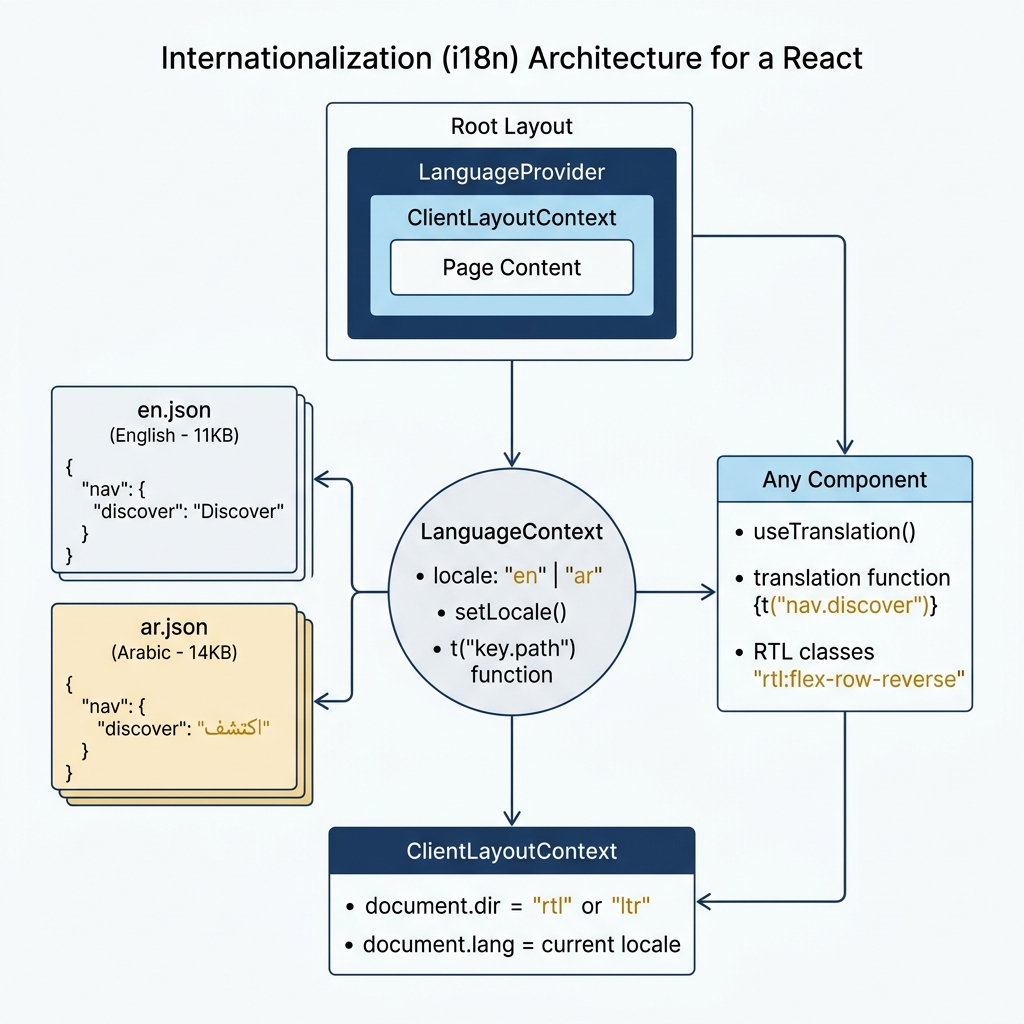
\includegraphics[width=0.9\textwidth]{images/i18n_architecture.png}
    \caption{i18n architecture — LanguageProvider supplies translations to all components via Context.}
\end{figure}

\subsection{Architecture}

The system consists of four parts:
\begin{itemize}[leftmargin=2em]
    \item \textbf{LanguageContext.tsx} — A React Context provider that holds the current locale and provides the \texttt{t()} translation function.
    \item \textbf{useTranslation.ts} — A convenience hook that wraps \texttt{useContext(LanguageContext)}.
    \item \textbf{Locale files} — \texttt{en.json} (11 KB) and \texttt{ar.json} (14 KB) containing all UI strings as nested JSON.
    \item \textbf{ClientLayoutContext} — Dynamically sets the HTML \texttt{dir} attribute to \texttt{"rtl"} or \texttt{"ltr"}.
\end{itemize}

\subsection{The Translation Function \texttt{t()}}

The \texttt{t()} function resolves dot-notation keys against the current locale's JSON file, with automatic fallback to English if a key is missing in Arabic:

\begin{lstlisting}[language=TypeScript,title={LanguageContext.tsx — Translation resolver (key logic)}]
const t = (key: string) => {
  const keys = key.split(".");
  let value: any = translations[locale];

  for (const k of keys) {
    if (value && typeof value === 'object' && k in value) {
      value = value[k];
    } else {
      // Fallback to English if key missing in Arabic
      let fallbackValue: any = translations["en"];
      for (const fk of keys) {
        fallbackValue = fallbackValue?.[fk];
      }
      return fallbackValue ?? key;
    }
  }
  return value;
};
\end{lstlisting}

\subsection{RTL Layout Switching}

The \texttt{ClientLayoutContext} component dynamically sets the document direction based on the active locale:

\begin{lstlisting}[language=TypeScript,title={ClientLayoutContext.tsx — RTL toggle}]
export const ClientLayoutContext = ({ children }) => {
  const { locale } = useTranslation();

  useEffect(() => {
    document.documentElement.dir = locale === "ar" ? "rtl" : "ltr";
    document.documentElement.lang = locale;
  }, [locale]);

  return <>{children}</>;
};
\end{lstlisting}

Throughout the codebase, Tailwind's \texttt{rtl:} modifier is used to flip padding, margins, and flex directions for Arabic layouts (e.g., \texttt{rtl:flex-row-reverse}, \texttt{rtl:right-4}).

% ══════════════════════════════════════════════════════════
% SECTION 9: CUSTOM HOOKS
% ══════════════════════════════════════════════════════════
\section{Custom Hooks}

Custom React hooks encapsulate reusable logic that can be shared across components. The project includes the \texttt{useScrollReveal} hook for scroll-triggered animations on the landing page.

\subsection{\texttt{useScrollReveal} — Intersection Observer}

This hook uses the browser's \texttt{IntersectionObserver} API to detect when an element enters the viewport, enabling reveal-on-scroll animations:

\begin{lstlisting}[language=TypeScript,title={useScrollReveal.ts — Complete implementation}]
"use client";
import { useEffect, useRef, useState } from "react";

export function useScrollReveal(threshold = 0.1) {
  const ref = useRef<HTMLDivElement>(null);
  const [isVisible, setIsVisible] = useState(false);

  useEffect(() => {
    const observer = new IntersectionObserver(
      ([entry]) => {
        setIsVisible(entry.isIntersecting);
      },
      { threshold }
    );

    const currentRef = ref.current;
    if (currentRef) observer.observe(currentRef);

    return () => {
      if (currentRef) observer.unobserve(currentRef);
    };
  }, [threshold]);

  return { ref, isVisible };
}
\end{lstlisting}

\textbf{Usage:} Components attach the \texttt{ref} to a container element and use \texttt{isVisible} to toggle CSS classes:

\begin{lstlisting}[language=TypeScript,title={Usage in a landing page section}]
const { ref, isVisible } = useScrollReveal();

return (
  <section ref={ref}
           className={`transition-all duration-700 ${
             isVisible ? "opacity-100 translate-y-0"
                       : "opacity-0 translate-y-8"
           }`}>
    {/* content */}
  </section>
);
\end{lstlisting}

% ══════════════════════════════════════════════════════════
% SECTION 10: ERROR HANDLING & PERFORMANCE
% ══════════════════════════════════════════════════════════
\section{Error Handling \& Performance Optimization}

\subsection{Error Handling}

Error handling is implemented at multiple levels across the frontend:

\subsubsection{API-Level Error Handling}

The centralized \texttt{apiClient} function wraps every API call in a \texttt{try/catch} block, ensuring network failures never crash the application. Every response follows the unified \texttt{APIResponse<T>} shape, so components always check \texttt{response.success} before using the data:

\begin{lstlisting}[language=TypeScript,title={Unified error handling pattern}]
const response = await apiClient<DataType>("/endpoint");

if (response.success && response.data) {
  // Handle success - update state with typed data
  setData(response.data);
} else {
  // Handle error - show user-friendly message
  setError(response.error || "Something went wrong");
}
\end{lstlisting}

\subsubsection{Form Validation}

Client-side validation runs before any API call, providing immediate feedback. The \texttt{LoginForm} and \texttt{RegisterForm} implement field-level validation with localized error messages:

\begin{lstlisting}[language=TypeScript,title={Client-side validation (from LoginForm.tsx)}]
const validate = () => {
  const newErrors: { email?: string; password?: string } = {};
  if (!formData.email)
    newErrors.email = t("auth.errors.emailRequired");
  else if (!/^\S+@\S+\.\S+$/.test(formData.email))
    newErrors.email = t("auth.errors.emailInvalid");
  if (!formData.password)
    newErrors.password = t("auth.errors.passwordRequired");

  setErrors(newErrors);
  return Object.keys(newErrors).length === 0;
};
\end{lstlisting}

Errors are displayed inline beneath each field via the \texttt{FormField} component's \texttt{error} prop, with a red border ring and error text. Field errors clear automatically when the user starts typing.

\subsubsection{Loading States}

Every page that fetches data displays a loading spinner while waiting for the API response, preventing users from seeing empty or broken layouts. A consistent pattern is used:

\begin{lstlisting}[language=TypeScript,title={Loading state pattern}]
const [loading, setLoading] = useState(true);

// In the render:
{loading ? (
  <div className="py-8 flex justify-center">
    <span className="material-symbols-outlined animate-spin">
      refresh
    </span>
  </div>
) : (
  // Render actual content
)}
\end{lstlisting}

\subsection{Performance Optimization}

\subsubsection{Next.js Image Optimization}

The \texttt{next/image} component is used for all images, providing automatic optimization, lazy loading, and responsive sizing:

\begin{lstlisting}[language=TypeScript,title={Optimized image loading}]
<Image src="/images/logo.png" alt="University Logo"
       width={64} height={64} className="object-contain" />
\end{lstlisting}

\subsubsection{Font Loading with \texttt{display: "swap"}}

Both fonts use \texttt{display: "swap"}, which shows fallback system fonts immediately and swaps to the custom font once loaded. This eliminates invisible text during font loading (FOIT — Flash of Invisible Text).

\subsubsection{Memoized Callbacks}

The \texttt{DashboardNavbar} uses \texttt{useCallback} to memoize the notification polling function, preventing unnecessary re-creation on every render:

\begin{lstlisting}[language=TypeScript,title={Memoized polling with cleanup}]
const fetchNotificationCount = useCallback(() => {
  apiClient<NotificationCount>("/notifications/count")
    .then((res) => {
      if (res.success && res.data) setNotifCount(res.data);
    });
}, []);

useEffect(() => {
  fetchNotificationCount();
  const interval = setInterval(fetchNotificationCount, 30000);
  return () => clearInterval(interval);  // Cleanup on unmount
}, [fetchNotificationCount]);
\end{lstlisting}

The \texttt{clearInterval} in the cleanup function ensures no memory leaks when the component unmounts.

\subsubsection{Scroll-Triggered Rendering}

The \texttt{useScrollReveal} hook (Section 9) uses the \texttt{IntersectionObserver} API instead of scroll event listeners, which is significantly more performant — the browser handles visibility detection natively without blocking the main thread.

% ══════════════════════════════════════════════════════════
% SECTION 11: KEY FEATURE PAGES WALKTHROUGH
% ══════════════════════════════════════════════════════════
\section{Key Feature Pages Walkthrough}

This section walks through three representative pages to demonstrate how all the concepts discussed above come together in practice.

\subsection{Landing Page (\texttt{/})}

The landing page is the public-facing marketing page that introduces the Sakny platform to prospective users.

% Uncomment the line below once you have the screenshot:
% \begin{figure}[H]
%     \centering
%     \includegraphics[width=\textwidth]{images/screenshot_landing.png}
%     \caption{Landing page — Hero section with call-to-action buttons.}
% \end{figure}

\textbf{Architecture:} The page is composed of 7 independent section components, each focused on a single visual block:

\begin{lstlisting}[language=TypeScript,title={page.tsx — Landing page composition}]
export default function Home() {
  return (
    <>
      <Navbar />
      <TrustBanner />
      <main className="flex-grow flex flex-col gap-32 pb-32">
        <Hero />
        <FeaturesGrid />
        <HowItWorks />
        <AIFeatures />
        <FinalCTA />
      </main>
      <Footer />
    </>
  );
}
\end{lstlisting}

\textbf{Key implementation details:}
\begin{itemize}[leftmargin=2em]
    \item Each section uses \texttt{useScrollReveal()} for reveal-on-scroll animations.
    \item All visible text is rendered through \texttt{t()} for bilingual support.
    \item The \texttt{Hero} component uses a background image with a gradient overlay (\texttt{bg-primary/80 mix-blend-multiply}) for a professional visual effect.
    \item The \texttt{Navbar} switches between transparent and glassmorphism styles based on scroll position using a scroll event listener.
\end{itemize}

\subsection{Student Dashboard (\texttt{/dashboard})}

The student dashboard is the main hub where students manage their housing journey.

% Uncomment the line below once you have the screenshot:
% \begin{figure}[H]
%     \centering
%     \includegraphics[width=\textwidth]{images/screenshot_dashboard.png}
%     \caption{Student dashboard — Welcome banner, document stepper, action cards, and deadlines panel.}
% \end{figure}

\textbf{Layout structure:} The page uses a 12-column CSS grid with the main content in 8 columns and a side panel in 4:

\begin{lstlisting}[language=TypeScript,title={DashboardPage.tsx — Grid layout structure}]
<div className="max-w-7xl mx-auto grid grid-cols-12 gap-8">
  {/* Left Column - 8 cols */}
  <div className="col-span-12 lg:col-span-8 space-y-12">
    <WelcomeBanner />
    <DocumentStatusStepper currentPhase={documentPhase} />
    <UploadDocumentCard onUploadSuccess={handleUploadSuccess} />
    {/* Quick Actions Grid */}
    <section className="grid grid-cols-1 md:grid-cols-2 gap-6">
      <ActionCard icon="assignment" title={t("dashboard.myApplication")} ... />
      <ActionCard icon="search" title={t("dashboard.findHousing")} ... />
      <ActionCard icon="group" title={t("dashboard.roommateMatching")} ... />
      <ActionCard icon="support_agent" title={t("dashboard.maintenanceRequest")} ... />
    </section>
  </div>
  {/* Right Column - 4 cols */}
  <div className="col-span-12 lg:col-span-4">
    <DeadlinesSidepanel />
  </div>
</div>
\end{lstlisting}

\textbf{Document Status Stepper:} A three-step progress indicator that dynamically updates based on the student's document verification status. The phase is computed from the API response:

\begin{lstlisting}[language=TypeScript,title={Document phase computation logic}]
const docs = res.data.documents;
if (docs.length === 0) setDocumentPhase("upload");
else if (docs.some(d => d.status === "pending"))
  setDocumentPhase("under_review");
else if (docs.every(d => d.status === "approved"))
  setDocumentPhase("approved");
else if (docs.some(d => d.status === "rejected"))
  setDocumentPhase("rejected");
\end{lstlisting}

\subsection{Messages Page (\texttt{/dashboard/messages})}

The messages page provides a student-to-administrator communication interface with a split-panel design.

% Uncomment the line below once you have the screenshot:
% \begin{figure}[H]
%     \centering
%     \includegraphics[width=\textwidth]{images/screenshot_messages.png}
%     \caption{Messages page — Conversation thread (left) and compose form (right).}
% \end{figure}

\textbf{Layout:} A 3-column grid where the conversation list takes 2 columns and the compose form takes 1:

\begin{lstlisting}[language=TypeScript,title={Messages page — Split panel layout}]
<div className="grid grid-cols-1 lg:grid-cols-3 gap-6">
  {/* Conversation Thread - 2/3 width */}
  <div className="lg:col-span-2 bg-white shadow-soft rounded-2xl">
    {messages.map((msg) => {
      const isMine = msg.sender_role === myRole &&
                     msg.sender_id === myId;
      return (
        <div className={`flex ${isMine ? "justify-end"
                                       : "justify-start"}`}>
          <div className={isMine
            ? "bg-primary text-white rounded-br-sm"
            : "bg-surface-container-low rounded-bl-sm"}>
            <div className="text-sm">{msg.body}</div>
            <div className="text-[10px] opacity-50">
              {new Date(msg.created_at).toLocaleString()}
            </div>
          </div>
        </div>
      );
    })}
  </div>
  {/* Compose Form - 1/3 width */}
  <div className="bg-white shadow-soft rounded-2xl p-6">
    <form onSubmit={handleSend}>
      {/* recipient, message body, send button */}
    </form>
  </div>
</div>
\end{lstlisting}

\textbf{Key implementation details:}
\begin{itemize}[leftmargin=2em]
    \item Messages are styled differently based on the sender — user's own messages are right-aligned with a primary blue background, while received messages are left-aligned with a light gray background (chat bubble pattern).
    \item Thread filtering: clicking a message from a specific user filters the view to show only that conversation thread.
    \item The scrollable message area uses \texttt{max-h-[500px] overflow-y-auto} for a fixed-height chat container.
    \item Empty states show a \texttt{forum} icon with ``No messages yet'' text, providing visual feedback instead of a blank area.
\end{itemize}

% ══════════════════════════════════════════════════════════
% SECTION 12: SUMMARY
% ══════════════════════════════════════════════════════════
\section{Summary}

The Sakny frontend was built as a modern, maintainable, and bilingual web application. The following table summarizes the key architectural decisions:

\begin{table}[H]
\centering
\begin{tabular}{@{}lp{8.5cm}@{}}
\toprule
\textbf{Aspect} & \textbf{Implementation} \\
\midrule
Framework & Next.js 16 with App Router (file-based routing, nested layouts) \\
Language & TypeScript 5 (static type safety) \\
Styling & Tailwind CSS 4 with custom design tokens (50+ semantic color tokens) \\
Routing & File-based routing with nested layouts for shared UI \\
State Management & React Context API (i18n) + local component state via hooks \\
API Communication & Centralized \texttt{apiClient<T>} wrapper with automatic JWT injection \\
Authentication & JWT stored in localStorage with role-based page guards \\
Internationalization & Context API + JSON locale files (EN/AR) + RTL layout switching \\
Icons & Material Symbols Outlined (Google Fonts) \\
Component Architecture & 3-layer: UI Primitives $\rightarrow$ Feature Components $\rightarrow$ Page Composition \\
Error Handling & Unified API response shape + client-side form validation + loading states \\
Performance & next/font swap, next/image optimization, IntersectionObserver, useCallback memoization \\
\bottomrule
\end{tabular}
\caption{Frontend architecture summary.}
\end{table}

The codebase consists of approximately 30+ routes, 25+ components, and supports full English/Arabic bilingual operation with automatic RTL layout switching — all built on a consistent design system with 6 reusable UI primitives.

\end{document}
